\documentclass{standalone}
\usepackage{graphicx}	
\usepackage{amssymb, amsmath, amsthm}
\usepackage{color}

\usepackage{tikz}
\usetikzlibrary{math, calc, arrows.meta}

\definecolor{light}{RGB}{220, 188, 188}
\definecolor{mid}{RGB}{185, 124, 124}
\definecolor{dark}{RGB}{143, 39, 39}
\definecolor{highlight}{RGB}{180, 31, 180}
\definecolor{gray10}{gray}{0.1}
\definecolor{gray20}{gray}{0.2}
\definecolor{gray30}{gray}{0.3}
\definecolor{gray40}{gray}{0.4}
\definecolor{gray60}{gray}{0.6}
\definecolor{gray70}{gray}{0.7}
\definecolor{gray80}{gray}{0.8}
\definecolor{gray90}{gray}{0.9}
\definecolor{gray95}{gray}{0.95}
  
\newcommand{\drawcube}[4]{
  \pgfmathsetmacro{\dx}{#1}
  \pgfmathsetmacro{\dy}{#2} 
  \pgfmathsetmacro{\dz}{#3}  
  \pgfmathsetmacro{\tilt}{#4}
  
  \fill[light]    ({-(1 - \tilt) * \dx}, -\dy + \dz) 
               -- ({(1 + \tilt) * \dx}, -\dy + \dz) 
               -- ({(1 - \tilt) * \dx}, \dy + \dz) 
               -- ({-(1 + \tilt) * \dx}, \dy + \dz) -- cycle;  

  \fill[mid]    ({-(1 - \tilt) * \dx}, -\dy) 
             -- ({-(1 - \tilt) * \dx}, -\dy + \dz)
             -- ({-(1 + \tilt) * \dx}, \dy + \dz) 
						 -- ({-(1 + \tilt) * \dx}, \dy) -- cycle;

  \fill[dark]    ({-(1 - \tilt) * \dx}, -\dy) 
              -- ({(1 + \tilt) * \dx}, -\dy)
              -- ({(1 + \tilt) * \dx}, -\dy + \dz) 
              -- ({-(1 - \tilt) * \dx}, -\dy + \dz) -- cycle;
                       
  \draw[dark]    ({(1 + \tilt) * \dx}, -\dy) 
              -- ({(1 + \tilt) * \dx}, -\dy + \dz) 
              -- ({(1 - \tilt) * \dx}, \dy + \dz) 
              -- ({-(1 + \tilt) * \dx}, \dy + \dz)
              -- ({-(1 + \tilt) * \dx}, \dy) 
              -- ({-(1 - \tilt) * \dx}, -\dy)
              -- cycle;
              
 \draw[dark]    ({-(1 + \tilt) * \dx + 0.01}, \dy + \dz) 
             -- ({-(1 - \tilt) * \dx + 0.01}, -\dy + \dz) 
             -- ({(1 + \tilt) * \dx + 0.01}, -\dy + \dz);
}

\newcommand{\drawcubecageback}[4]{
  \pgfmathsetmacro{\dx}{#1}
  \pgfmathsetmacro{\dy}{#2} 
  \pgfmathsetmacro{\dz}{#3}  
  \pgfmathsetmacro{\tilt}{#4}
                   
  \draw[dark, dashed]    ({(1 - \tilt) * \dx}, \dy) 
                      -- ({(1 - \tilt) * \dx}, \dy + \dz) 
                      -- ({-(1 + \tilt) * \dx}, \dy + \dz) 
                      -- ({-(1 + \tilt) * \dx}, \dy) 
                      -- cycle;
}

\newcommand{\drawcubecagefront}[4]{
  \pgfmathsetmacro{\dx}{#1}
  \pgfmathsetmacro{\dy}{#2} 
  \pgfmathsetmacro{\dz}{#3}  
  \pgfmathsetmacro{\tilt}{#4}
                   
  \draw[dark, dashed]    ({(1 + \tilt) * \dx}, -\dy) 
                      -- ({(1 + \tilt) * \dx}, -\dy + \dz) 
                      -- ({-(1 - \tilt) * \dx + 0.015}, -\dy + \dz) 
                      -- ({-(1 - \tilt) * \dx + 0.015}, -\dy) 
                      -- cycle;
                      
  \draw[dark, dashed]    ({-(1 + \tilt) * \dx + 0.01}, \dy + \dz) 
                      -- ({-(1 - \tilt) * \dx + 0.01}, -\dy + \dz);

  \draw[dark, dashed]    ({(1 - \tilt) * \dx}, \dy + \dz) 
                      -- ({(1 + \tilt) * \dx}, -\dy + \dz);
             
}

\begin{document}

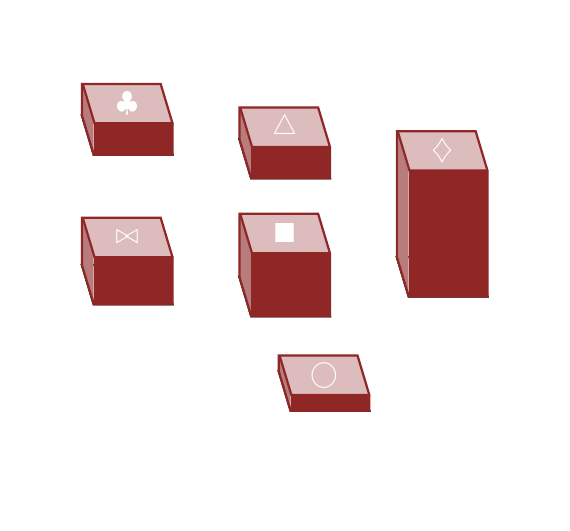
\begin{tikzpicture}[scale=1, thick]

  \draw[white] (-3.25, -3) rectangle (3.25, 3);
  
  \pgfmathsetmacro{\dx}{0.5}
  \pgfmathsetmacro{\dy}{0.25}
  \pgfmathsetmacro{\tilt}{0.3 * \dy / \dx}

  \foreach \x/\y\glyph [count=\n] in {0/-0.4/\blacksquare, -2/1.65/\clubsuit, 2/-0.15/\diamondsuit, 
                                      0.5/-1.6/\bigcirc, 0/1.35/\triangle, -2/-0.25/\bowtie} {
    \begin{scope}[shift={(\x, \y)}]
      \filldraw[fill=white, draw=black]    
           ({-(1 - \tilt) * \dx}, -\dy) -- ({(1 + \tilt) * \dx}, -\dy) 
        -- ({(1 - \tilt) * \dx}, \dy) -- ({-(1 + \tilt) * \dx}, \dy) -- cycle;
      \node at (0, 0) { $\glyph$ };
    \end{scope}
  } 
  
  \pgfmathsetmacro{\dx}{0.5}
  \pgfmathsetmacro{\dy}{0.25}
  \pgfmathsetmacro{\tilt}{0.3 * \dy / \dx}
  \foreach \x/\y/\p\glyph [count=\n] in {0/-0.4/0.2/\blacksquare, -2/1.65/0.1/\clubsuit, 2/-0.15/0.4/\diamondsuit, 
                                         0.5/-1.6/0.05/\bigcirc, 0/1.35/0.1/\triangle, -2/-0.25/0.15/\bowtie} {
    \begin{scope}[shift={(\x, \y)}]
      \drawcube{\dx}{\dy}{4 * \p}{\tilt}
      \node[white] at (0, {4 * \p}) { $\glyph$ };
    \end{scope}
  }
 
  
\end{tikzpicture}

\end{document}  